\section{磁链与自感系数}

电流产生磁场，电流变化也会改变穿过电路自身的磁通。对于固定形状、线性介质中的线圈，各匝磁通之和称为磁链 $\Psi$。若它与电流成正比，定义 $\Psi=Li$。这里已经把匝数包含在磁链内，不能再把 $N$ 重复乘到电动势公式中。自感电动势为 $\varepsilon_L=-\dot\Psi=-L\dot i$；按电流流入端为正端定义线圈电压，则 $u_L=L\dot i$。

负号阻碍的是电流变化，并非总与电流反向。电流正在减小时，自感作用继续维持原电流，线圈把磁场能送回电路；电流正在增大时，电源须克服这一作用，磁场储能增加。线圈不是恒定电阻，瞬时比值 $u_L/i$ 不能作为自感系数，其量纲也不对。$L$ 的单位是亨利，等于伏秒每安。

长螺线管内部磁场近似 $B=\mu Ni/\ell$，单匝磁通为 $BS$，磁链 $NBS=\mu N^2Si/\ell$，从而
\begin{equation}L=\frac{\mu N^2S}{\ell}.\label{em4:solenoid}\end{equation}

这要求线圈足够长、内部场近似均匀、漏磁可以忽略，介质磁导率不随场显著变化。若磁芯饱和，$\Psi(i)$ 不再是直线，暂态关系应写成 $u=\dd\Psi/\dd t$，不能把一个固定 $L$ 用到底。几何改变时，$L$ 也会变化，此时 $\dot\Psi=L\dot i+i\dot L$，后一项不能漏掉。

\fig{em4:coil}{线圈纵截面中的电流方向与轴向磁场；右图为从右端观察的截面}{\begin{tikzpicture}

\draw[world](0,0)rectangle(4,1.4);
\foreach \x in {.3,.8,1.3,1.8,2.3,2.8,3.3,3.8}{\node at(\x,1.4){$\odot$};\node at(\x,0){$\otimes$};}
\draw[flow,blue](.3,.7)--(3.7,.7)node[midway,above]{$\bm B$};
\draw[dim](0,-.55)--(4,-.55)node[midway,below]{$\ell$};\node at(2,2){$N$ 匝};
\draw[axis](3,2.55)--(4.2,2.55)node[right]{$+x$};
\begin{scope}[xshift=6cm]\fill[blue!10](0,.7)circle(.8);\draw[world](0,.7)circle(.8);
\node at(0,.7){$\odot B$};\draw[flow,red](.566,1.266)arc(45:145:.8);\node at(0,-.6){截面积 $S$};\end{scope}

\end{tikzpicture}}


图\ref{em4:coil}中的长度 $\ell$决定单位长度匝数，截面积 $S$决定单匝磁通，再乘总匝数 $N$才得磁链。因此自感随 $N^2$变化：一因子来自励磁场，另一因子来自链接磁通的匝数，不能把磁通与磁链都重复乘匝数。


\section{从建立电流的过程得到磁场能量}

把理想电感接到外电源上，缓慢建立电流。电源克服线圈端电压所做的微元功为 $\dd W=u_Li\dd t=Li\dd i$。从零电流积分到 $I$，得到
\begin{equation}W_B=\int_0^I Li\dd i=L\left[\frac{i^2}{2}\right]_0^I=\frac12LI^2.\label{em4:energy}\end{equation}
若还串有电阻，电源功同时分为磁场能增量与焦耳热，不能把输入电能全部认作磁能。磁场能在电流为负时仍为正；只要电流绝对值增加，磁场能就增加。

将螺线管的 $L$ 与 $B$ 代入，$W_B=B^2S\ell/(2\mu)$。在均匀线性介质中，单位体积磁能密度因此为 $w_B=B^2/(2\mu)$。非均匀场需要对全空间积分，不能只取导线内部或者只取磁感应强度最大的区域。孤立细圆环的外部磁场通常占主要部分，不能直接把环内面积乘一个处处相同的中心磁场来算精确自感。

能量法还揭示了电感电流的连续性。对电压积分有 $L[i(t_2)-i(t_1)]=\int_{t_1}^{t_2}u\dd t$。若切换时间趋零而电压没有冲激，积分趋零，电流不能突变。要在理想零时间内突然切断有限电感电流，就要求无穷电压；真实电路会经寄生电容、火花或其他通路释放磁能。不能同时假设电流瞬间归零、电压有限和磁能没有去处。


\fig{em4:current-voltage}{被动端压的正端是电流流入端；端压符号由磁链斜率决定}{\begin{tikzpicture}

\draw[world](0,2.4)--(0,1.95);\foreach \j in {0,...,3}{\draw[world](0,{.35+.4*\j})arc(-90:90:.2);}\draw[world](0,.35)--(0,0);
\node[left]at(-.35,2.35){$+$};\node[left]at(-.35,0){$-$};\node[left]at(-.5,1.1){$u_L$};\node[right]at(.4,1.1){$L$};\draw[flow,red](0,3)--(0,2.45)node[midway,right]{$i$};
\begin{scope}[xshift=3cm]
\draw[axis](-.2,0)--(5.5,0)node[right]{$t$};\draw[axis](0,-.2)--(0,2.1)node[above]{$i$};
\draw[world,blue](0,0)--(1,1.6)--(3,1.6)--(5,0);\node[left]at(0,1.6){$I$};
\foreach \x/\txt in {1/T,3/3T,5/5T}{\draw[guide](\x,0)--(\x,-.8);\node[below]at(\x,0){$\txt$};}
\draw[axis](-.2,-2)--(5.5,-2)node[right]{$t$};\draw[axis](0,-2.85)--(0,-.95)node[above]{$u_L$};
\draw[red,thick](0,-1.15)--(1,-1.15) (1,-2)--(3,-2) (3,-2.425)--(5,-2.425);
\node[left]at(0,-1.15){$LI/T$};\node[left]at(0,-2.425){$-LI/(2T)$};\end{scope}

\end{tikzpicture}}

图\ref{em4:current-voltage}的上图先使电流线性增大，再保持，最后缓慢减小。三段斜率依次为 $I/T,0,-I/(2T)$，因此下图端压为 $LI/T,0,-LI/(2T)$。下降段仍有正向电流，却有负端压，功率 $u_Li<0$，表示磁场向外送能。转折处只是斜率改变，电流本身连续；图中的有限电压阶跃并不造成电流突变。


\section{磁链法与场能法的相互验证}

自感可以由磁链除以电流求出，也可以先积分磁场能再与 $LI^2/2$ 比较。前者要求辨认每一匝实际链接的磁通，后者要求包含所有显著场能区域。二者使用同一模型边界时必须一致；若不一致，往往是漏算匝数、漏算外部磁场，或把并非全部链接的磁通当成全部链接。

以理想同轴结构为例，内导体半径 $a$、外导体内半径 $b$，两导体电流等大反向。忽略端部及导体内部磁场，安培定律给出 $a<s<b$ 中 $B(s)=\mu I/(2\pi s)$。长度 $\ell$ 的薄圆柱壳体积为 $2\pi s\ell\dd s$，所以
\[W_B=\int_a^b\frac{B(s)^2}{2\mu}2\pi s\ell\dd s
=\frac{\mu I^2\ell}{4\pi}\int_a^b\frac{\dd s}{s}
=\frac{\mu I^2\ell}{4\pi}[\ln s]_a^b
=\frac{\mu I^2\ell}{4\pi}\ln\frac ba.\]

与磁能式比较，单位长度外自感为 $L'=\mu\ln(b/a)/(2\pi)$。对每一条与轴平行、从内导体延伸到外导体的窄带积分磁通，也得到 $\Psi=\mu I\ell\ln(b/a)/(2\pi)$，结果一致。若直流电流均匀分布于内导体截面，内部还会有额外自感；本式没有包含它，不能声称适用于所有频率的完整电缆自感。

\fig{em4:coax-flux}{同轴结构的环向磁场；磁通积分取径向与轴向组成的窄带}{\begin{tikzpicture}

\fill[blue!8,even odd rule](0,0)circle(1.65)(0,0)circle(.65);
\draw[world](0,0)circle(.65)(0,0)circle(1.65);\node at(0,0){$\odot I$};
\draw[guide](0,0)circle(1.15);\draw[flow,blue](.813,.813)arc(45:140:1.15);\node[above]at(-.8,1.1){$B(s)$};
\draw[dim](0,0)--(.65,0)node[midway,below]{$a$};\draw[dim](0,0)--(0,-1.65)node[midway,left]{$b$};\node at(0,-2.3){外导体回流 $\otimes I$};
\begin{scope}[xshift=4cm]
\draw[axis](0,0)--(3.8,0)node[right]{$s$};\draw[axis](0,0)--(0,2.3)node[above]{$z$};
\fill[blue!12](.7,0)rectangle(3,1.8);\draw[world](.7,0)rectangle(3,1.8);
\fill[blue!40](1.7,0)rectangle(1.9,1.8);\draw[guide](1.7,0)--(1.7,-.6);
\node[below]at(.7,0){$a$};\node[below]at(3,0){$b$};\node at(2.5,.9){$\otimes B$};\node[left]at(.7,.9){$\ell$};
\node at(1.8,-.9){$\dd S=\ell\dd s$};\end{scope}

\end{tikzpicture}}

图\ref{em4:coax-flux}左图说明 $B$ 沿圆周而变，右图所取的径向—轴向窄带才与 $B$ 垂直。单个同轴回路由内导体前行、外导体回行，所围跨接面为这条窄带，故 $\dd\Psi=B(s)\ell\dd s$。能量积分使用的体积元却是整圈圆柱壳 $2\pi s\ell\dd s$；面积元和体积元不能相互替代。


环形螺线管则说明“平均半径”只是近似。截面为高 $h$、内外半径 $a,b$ 的矩形环形线圈有 $B(s)=\mu NI/(2\pi s)$，单匝磁通用截面窄条积分为
\[
\Phi=\frac{\mu NIh}{2\pi}\int_a^b\frac{\dd s}{s}
=\frac{\mu NIh}{2\pi}[\ln s]_a^b
=\frac{\mu NIh}{2\pi}\ln\frac ba,
\]因此 $L=\mu N^2h\ln(b/a)/(2\pi)$。只有当径向宽度远小于平均半径时，才能用平均周长与近似均匀磁场化成通常的长螺线管形式。


\fig{em4:toroid-strip}{环形线圈的环向场与矩形截面；各径向位置的场强不同}{\begin{tikzpicture}

\fill[gray!12,even odd rule](0,0)circle(1.6)(0,0)circle(.8);\draw[world](0,0)circle(1.6)(0,0)circle(.8);
\draw[flow,blue](1.2,0)arc(0:135:1.2);\node at(-.2,1.9){$B(s)$};
\draw[dim](0,0)--(.8,0)node[midway,below]{$a$};\draw[dim](0,0)--(0,-1.6)node[midway,left]{$b$};\node at(0,-2.2){密绕 $N$ 匝};
\begin{scope}[xshift=4cm]
\draw[world](0,0)rectangle(3,1.8);\fill[blue!30](1.3,0)rectangle(1.5,1.8);\draw[dim](-.5,0)--(-.5,1.8)node[midway,left]{$h$};
\draw[axis](-.2,-.45)--(3.5,-.45)node[right]{$s$};\node[below]at(0,-.45){$a$};\node[below]at(3,-.45){$b$};
\node at(2.3,.9){$\otimes B(s)$};\node at(1.4,2.25){$\dd s$};\draw[guide](1.4,2)--(1.4,1.8);\node at(1.5,-1.25){$\dd\Phi=B(s)h\dd s$};\end{scope}

\end{tikzpicture}}
沿图\ref{em4:toroid-strip}右图从 $a$ 积分到 $b$，再乘链接这些磁通的 $N$ 匝，才得到磁链。令 $r_m=(a+b)/2,w=b-a$，当 $w/r_m\ll1$，
令 $x=w/(2r_m)$，为说明近似误差，定义 $G(x)=\ln(1+x)-\ln(1-x)$。
在 $|x|<1$ 内逐项求导并作精确分解，
\[
 G'(x)=\frac1{1+x}-\frac{-1}{1-x}
 =\frac2{1-x^2}=2(1+x^2)+\frac{2x^4}{1-x^2}.
\]
由 $G(0)=0$，积分回去，
\[
 \begin{aligned}
 G(x)&=2\int_0^x(1+u^2)\dd u
       +2\int_0^x\frac{u^4}{1-u^2}\dd u\\
 &=2[u+u^3/3]_0^x+O(x^5)=2x+\frac{2x^3}{3}+O(x^5).
 \end{aligned}
\]
第二个积分的分母在零点附近有界且不为零，故余项为五阶。代回宽度，
\[
 \ln\frac ba=\frac w{r_m}+\frac{w^3}{12r_m^3}
 +O\!\left(\frac{w^5}{r_m^5}\right).
\]
保留首项便有 $L\simeq\mu N^2hw/(2\pi r_m)$，即截面积 $S=hw$、平均磁路长 $2\pi r_m$ 的均匀场近似。对称取平均半径后相对误差从 $(w/r_m)^2$ 阶开始，宽环不能直接忽略。


\section{有气隙磁路的磁链与能量分布}

磁芯把磁场集中在一个近似闭合通道中，但气隙会显著改变自感。若截面积 $S$ 近似恒定、漏磁与边缘扩展可以忽略，磁通连续性给出磁芯和气隙中的 $B=\Phi/S$ 相同。沿磁路使用安培定律，$H_c\ell+H_gg=Ni$；在线性介质中 $H_c=B/\mu,H_g=B/\mu_0$，因此
\[Ni=\Phi\left(\frac{\ell}{\mu S}+\frac g{\mu_0S}\right).\]
括号称为磁阻。它描述磁通与磁动势的比例，不是导线电阻，不会因此产生 $i^2R$ 式焦耳热。由 $\Psi=N\Phi$ 可得 $L=N^2/[\ell/(\mu S)+g/(\mu_0S)]$。即使气隙很短，因为 $\mu\gg\mu_0$，气隙项仍可能主导总磁阻。

场能密度分别为 $B^2/(2\mu)$、$B^2/(2\mu_0)$。同样的 $B$ 下，气隙单位体积的能量远大于磁芯中。铁芯导磁并不意味着主要磁能都储存在铁芯内；在有明显气隙的电磁铁中，许多磁能实际储存在空气间隙。用气隙能随宽度变化计算吸力时，还必须保留固定电流或固定磁链的控制条件。

\fig{em4:growth:gap}{磁通连续的磁芯与气隙}{\begin{tikzpicture}[scale=.88]\path[fill=gray!18,even odd rule](0,0)rectangle(4,3) (.6,.6)rectangle(3.4,2.4);\draw[world](0,0)rectangle(4,3) (.6,.6)rectangle(3.4,2.4);\fill[white](1.8,2.35)rectangle(2.2,3.05);\draw[world](1.8,2.4)--(1.8,3) (2.2,2.4)--(2.2,3);\draw[dim](1.8,3.4)--(2.2,3.4)node[midway,above]{$g$};\foreach\y in{1,1.2,1.4,1.6,1.8,2}{\draw[world](-.2,\y)--(.8,\y);}\node[left]at(-.3,1.5){$N,i$};\draw[flow](1,.3)--(2.8,.3)node[midway,above]{$\Phi$};\end{tikzpicture}}


图\ref{em4:growth:gap}中同一磁通依次穿过磁芯和气隙，因此安培积分沿这两段串行相加。气隙长度虽短，$\mu_0$却小，往往主导磁阻和储能。改变气隙时，还应说明电流由电源保持，还是闭合回路保持磁链，再据此计算机械功。



若磁芯和气隙截面积相同，两部分总能量之比还可直接写为
\[\frac{W_g}{W_c}=\frac{g/\mu_0}{\ell/\mu}=\frac{\mu g}{\mu_0\ell}.\]
这与各段磁阻之比相同。图\ref{em4:growth:gap}中穿过气隙的磁通沿上支路向左，密度仍为 $B=\Phi/S$；气隙并未凭空增加磁通，而是要求更大的励磁安匝数。以上结论依赖漏磁及边缘扩展可忽略，气隙接近横截面尺度时要重新求场。


\section{电流分布、内部自感与非线性磁链}

同轴结构的外部自感只涉及两导体之间的磁场。若导体内部电流均匀分布，安培环路包围的电流随半径平方增加，导体内部也有磁场和磁能。高频集肤时电流向表面集中，内部场能减小，所以同一几何结构在不同电流分布条件下的总自感可以不同。本讲用均匀直流电流分布求内部项，并与已得到的外部项相加，两个区域的积分边界不能重叠。


取内导体磁导率为 $\mu_c$、间隙介质为 $\mu_m$，在半径 $s<a$ 的环路内，电流为 $I_s=Is^2/a^2$，所以
\[B_{\rm in}(s)=\frac{\mu_cIs}{2\pi a^2},\qquad
W'_{\rm in}=\int_0^a\frac{B_{\rm in}^2}{2\mu_c}2\pi s\dd s
=\frac{\mu_cI^2}{4\pi a^4}\int_0^a s^3\dd s
=\frac{\mu_cI^2}{4\pi a^4}\left[\frac{s^4}{4}\right]_0^a
=\frac{\mu_cI^2}{16\pi}.\]
撇号表示单位轴向长度。由 $W'_{\rm in}=L'_{\rm in}I^2/2$，得 $L'_{\rm in}=\mu_c/(8\pi)$，与外部项相加为
\[L'_{\rm total}=\frac{\mu_c}{8\pi}+\frac{\mu_m}{2\pi}\ln\frac ba.\]
外回流层自身的内部场仍未计入。几何放大使内部场按长度的倒数减弱，单位长度体积却按长度平方增加，所以给定 $I$ 时内部储能不随 $a$ 改变。
\fig{em4:internal-profile}{均匀直流电流的内部场与同轴间隙中的外部场；图取相同磁导率}{\begin{tikzpicture}

\draw[axis](-.2,0)--(5.8,0)node[right]{$s/a$};\draw[axis](0,-.2)--(0,2.6)node[above]{$B/B(a)$};
\fill[blue!12](0,0)--(2,2)--(2,0)--cycle;\draw[world,blue](0,0)--(2,2);
\draw[world,red,domain=2:5,samples=60]plot(\x,{4/\x});\draw[guide](2,0)--(2,2)--(0,2);
\draw[world,red](5,0)--(5.5,0);\draw[guide](5,0)--(5,.8);
\node[below]at(2,0){$1$};\node[below]at(5,0){$b/a$};\node[left]at(0,2){$1$};
\node at(1,2.5){$B\propto s$};\node at(3.6,2.1){$B\propto1/s$};\node at(3,-.9){薄回流层外净包围电流为零};

\end{tikzpicture}}

图\ref{em4:internal-profile}的两段积分边界恰在 $s=a$ 连接。图中为 $\mu_c=\mu_m$ 的特例；若磁导率不同，切向 $H$ 在没有表面电流的界面连续，$B$ 可以跳变，不能强行沿用图中的连续曲线。


对可逆但非线性的磁环境，自感不能只用一个常数表示。应将磁链写为 $\Psi(i)$，电压 $u=\dot\Psi$，微元输入功为 $i\dd\Psi$，场能为 $W(\Psi)=\int_0^\Psi i(\psi)\dd\psi$。只有 $i=\Psi/L$ 为直线时，积分才化成 $Li^2/2$。瞬时增量电感 $L_d=\dd\Psi/\dd i$ 与从原点连到当前点的比值 $\Psi/i$ 一般不同，暂态斜率需要前者。

若磁芯存在磁滞，建立和撤去电流的路径不同，输入功与可回收储能也要区分。这里的非线性例题明确采用单值、可逆关系，不能把其全部输入功公式直接用于有磁滞损耗的铁磁循环。模型条件决定能量积分的含义，不能用同一个“自感”符号掩盖不同物理过程。

\fig{fv:f4:nonlinear}{非线性可逆磁链中，场能是电流对磁链的积分}{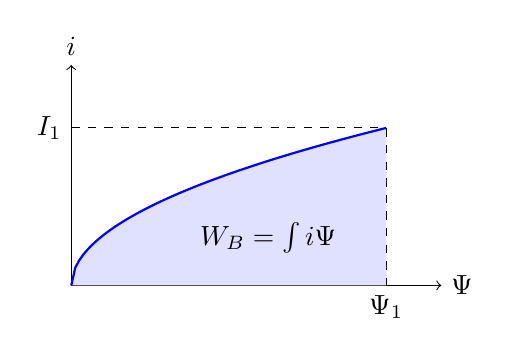
\begin{tikzpicture}[x=1cm,y=1cm]
\draw[->](0,0)--(4.7,0)node[right]{$\Psi$};\draw[->](0,0)--(0,2.8)node[above]{$i$};
\fill[blue!12](0,0)--plot[domain=0:4,samples=80](\x,{sqrt(\x)})--(4,0)--cycle;
\draw[blue,thick,domain=0:4,samples=80]plot(\x,{sqrt(\x)});\draw[dashed](0,2)--(4,2)--(4,0);
\node[below]at(4,0){$\Psi_1$};\node[left]at(0,2){$I_1$};\node at(2.5,.6){$W_B=\int i\dd\Psi$};\end{tikzpicture}}
图\ref{fv:f4:nonlinear}把磁链作为横坐标，蓝色面积才直接等于输入功。取 $i\ge0$区间内的示例 $\Psi=\alpha i^2$，反解 $i(\psi)=\alpha^{-1/2}\psi^{1/2}$，就有
\[
W_B=\alpha^{-1/2}\int_0^{\Psi_1}\psi^{1/2}\dd\psi
=\alpha^{-1/2}\left[\frac23\psi^{3/2}\right]_0^{\Psi_1}
=\frac23I_1\Psi_1,
\]并非 $I_1\Psi_1/2$。矩形剩余面积称磁共能 $W_B^*=\int_0^{I_1}\Psi(i)\dd i=I_1\Psi_1-W_B$，通常与场能不同。可逆系统有 $\dd W_B=i\dd\Psi-F\dd x$，因此 $\dd W_B^*=\Psi\dd i+F\dd x$：固定电流求力时应取 $F=\partial W_B^*/\partial x|_i$，固定磁链时取 $F=-\partial W_B/\partial x|_\Psi$。线性关系恰好把矩形分成两半，才有熟悉的二分之一系数；有磁滞时还须区分进入与返回路径，不能按单值曲线积分。



\section{互感、同名端与耦合能量}

两个固定线圈处在线性磁环境中时，分别选择参考电流方向，可将磁链写为
\[\Psi_1=L_1i_1+Mi_2,\qquad \Psi_2=Mi_1+L_2i_2.\]
互感系数在互易的线性系统中相同，符号由方向约定决定。图中的小圆点称同名端：若两个参考电流都流入同名端，取 $M>0$，相互产生的磁链沿各自正向。反接一个线圈相当于改变互感项的符号，几何距离并未改变，不能说反接后耦合程度就消失。

\fig{em4:dots}{两个参考电流均流入同名端，电压均按被动约定取正}{\begin{tikzpicture}

\foreach \x/\j in {0/1,3.5/2}{
\draw[world](\x,2.4)--(\x,1.95);\foreach \n in {0,...,3}{\draw[world](\x,{.35+.4*\n})arc(-90:90:.2);}\draw[world](\x,.35)--(\x,0);
\fill({\x-.25},2.15)circle(2pt);\node[left]at(\x,1.1){$L_{\j}$};\draw[flow,red](\x,3.1)--(\x,2.5)node[midway,right]{$i_{\j}$};
\node[right]at({\x+.3},2.35){$+$};\node[right]at({\x+.3},0){$-$};}
\draw[<->](.8,1.1)--(2.8,1.1)node[midway,above]{$M>0$};

\end{tikzpicture}}


图\ref{em4:dots}的两个参考电流都流入圆点端，所以磁链式的互感项同取正号。若实际反接一个绕组，而外部端口的电压、电流参考保持原约定，互感项应变号。若只是反选某一绕组的参考方向，则该绕组的电流、电压和磁链变量都变号，互感的有向系数也相应改变。实际接线变化与坐标重选必须区分，功率 $ui$ 在自洽的参考变换下不变。


端电压为磁链的时间导数。建立两电流时，展开输入微元功，
\[
\dd W=L_1i_1\dd i_1+L_2i_2\dd i_2
+M(i_1\dd i_2+i_2\dd i_1).
\]
末两项由乘积微分合为 $M\dd(i_1i_2)$；前两项各以平方的一半为原函数。从两电流均为零积到 $(i_1,i_2)$，端点代入为
\[
 W_B=\frac{L_1}{2}[z^2]_0^{i_1}
    +\frac{L_2}{2}[y^2]_0^{i_2}
    +M[i_1i_2]_{(0,0)}^{(i_1,i_2)}.
\]
因此
\[W_B=\frac12L_1i_1^2+\frac12L_2i_2^2+Mi_1i_2.\]
交叉项既可为正，也可为负，整个磁能仍不能为负。固定 $i_2$，把 $i_1$ 配方，可写成
\[W_B=\frac{L_1}{2}\left(i_1+\frac{M}{L_1}i_2\right)^2+\frac12\left(L_2-\frac{M^2}{L_1}\right)i_2^2.\]
因此 $M^2\le L_1L_2$。定义耦合系数 $k=M/\sqrt{L_1L_2}$，它的绝对值不超过一。接近一意味着漏磁很小，不意味着电阻或铁芯损耗也为零。

串联两线圈时，先按同名端判断两互感电压相加还是相减，再得到 $L_s=L_1+L_2\pm2M$。并联则不能把两个串联公式倒过来使用，因为支路电流一般不相等。应令两支路端电压相同，联立含互感的方程，再用总电流定义等效电感。反向并联的相同绕组在完全耦合极限下具有零端口电感，外加有限电压时电流增长由真实漏感与电阻限制。匝数不同的完全耦合绕组直接同名端并联，则是端电压约束与匝数比不相容，可能出现很大的环流；两种情形不能混为同一种退化原因。

\section{不等线圈的连接与参考方向}

两个不相同的线圈同名端并联，电压分别为 $u=L_1\dot i_1+M\dot i_2$、$u=M\dot i_1+L_2\dot i_2$。令 $D=L_1L_2-M^2>0$。第一式乘 $L_2$、第二式乘 $M$ 后相减，消去 $\dot i_2$；再交换消元对象，得到
\[
 \begin{aligned}
 (L_2-M)u&=L_1L_2\dot i_1+ML_2\dot i_2
              -M^2\dot i_1-ML_2\dot i_2=D\dot i_1,\\
 (L_1-M)u&=D\dot i_2.
 \end{aligned}
\]
因此 $\dot i_1=u(L_2-M)/D$、$\dot i_2=u(L_1-M)/D$，总电流导数为 $u(L_1+L_2-2M)/D$，所以
\[L_p=\frac{L_1L_2-M^2}{L_1+L_2-2M}.\]
反接一组后按新方向重新定义互感项，相当于将式中的 $M$ 换为 $-M$。不能对不等线圈先假定两支路各分一半电流；当某一系数使导数为负，可能出现反向的环流分量，这需要根据初始电流与电源端口共同解释。

完全耦合时 $D=0$，上述除以 $D$ 的推导不适用。尤其是匝数不同的理想完全耦合绕组直接并联，要求相同端电压又要求电压按匝数成比例，理想约束互相矛盾。真实漏感和电阻会产生很大环流，不能把零分子当成“等效电感为零，所以任意并联都可行”。相同绕组的完全耦合是特殊退化情形：端口关系存在，但支路差模电流须由初态或实际非理想因素另行确定。

同名端可用实验定义而不依赖绕线图的外观。向第一线圈同名端注入一个增长电流，若第二线圈按流入其同名端的被动端压为正，则两端为同名。第二线圈接电阻闭合时，感应电流往往从同名端流出，以阻碍初级磁链增长，这与开路感应电压的正端并不矛盾。


\fig{em4:parallel-example}{同名端并联可有相反的支路电流变化率；图示零初态加恒定正电压}{\begin{tikzpicture}

\draw[world](0,2.4)--(0,2.8)--(2.6,2.8)--(2.6,2.4) (0,0)--(0,-.4)--(2.6,-.4)--(2.6,0);
\foreach \x in {0,2.6}{\draw[world](\x,2.4)--(\x,1.95);\foreach \n in {0,...,3}{\draw[world](\x,{.35+.4*\n})arc(-90:90:.2);}\draw[world](\x,.35)--(\x,0);\fill({\x-.23},2.15)circle(2pt);}
\node[left]at(0,1.1){$4L_0$};\node[right]at(3,1.1){$L_0$};\fill(1.3,2.8)circle(2pt)node[above]{$A$};\fill(1.3,-.4)circle(2pt)node[below]{$B$};\node at(1.3,1.1){$M=1.5L_0$};
\draw[flow](-.6,2.6)--(-.6,1.9)node[left]{$i_1$};\draw[flow](3.6,2.6)--(3.6,1.9)node[right]{$i_2$};
\begin{scope}[xshift=5cm]
\draw[axis](-.2,0)--(3,0)node[right]{$ut/L_0$};\draw[axis](0,-1)--(0,4.35)node[above]{$i_1,i_2$};
\draw[blue,thick](0,0)--(2.7,{2.7*10/7});\draw[red,thick](0,0)--(2.7,{-2.7*2/7});
\node[right]at(2.7,{2.7*10/7}){$i_2$};\node[right]at(2.7,{-2.7*2/7}){$i_1$};\end{scope}

\end{tikzpicture}}
例如图\ref{em4:parallel-example}中 $D=(7/4)L_0^2>0$，代入得 $\dot i_1=-2u/(7L_0)$、$\dot i_2=10u/(7L_0)$。支路一的电流从零向负方向增长，但总电流导数为 $8u/(7L_0)>0$，端口等效电感为 $7L_0/8$，并不违反被动系统的能量约束。互感传能使单支路的变化方向不能仅由该支路端压判断。

对相同绕组的完全同向耦合，端口仍有 $L_p=L$，但方程只决定 $i_1+i_2$，不决定无磁场的差模电流 $i_1-i_2$。只有对称初态或其他给定约束才能令两者相等；不能把均分电流当成所有初态都成立的结论。


\section{磁耦合的反馈、屏蔽与模态}

闭合次级线圈中的感应电流会反馈到初级磁链。若次级超导、初始次级总磁链为零，约束为 $Mi_1+L_2i_2=0$。代入初级磁链后，端口等效自感减为 $L_1-M^2/L_2$。减少的不是导线本身的匝数，而是次级感应磁场抵消了初级一部分磁链。这个结果与耦合能量的非负条件相容，等效自感不会为负。

\fig{em4:screen-secondary}{闭合超导次级的实际电流从同名端流出，抵消次级的总磁链变化}{\begin{tikzpicture}

\foreach \x/\j in {0/1,3/2}{\draw[world](\x,2.4)--(\x,1.95);\foreach \n in {0,...,3}{\draw[world](\x,{.35+.4*\n})arc(-90:90:.2);}\draw[world](\x,.35)--(\x,0);\fill({\x-.22},2.15)circle(2pt);\node[left]at(\x,1.1){$L_{\j}$};}
\draw[world](3,2.4)--(4.4,2.4)--(4.4,0)--(3,0);\draw[flow,red](0,3.1)--(0,2.5)node[midway,left]{$i_1>0$};\draw[flow,blue](3,2.45)--(3,3.1)node[above]{$|i_2|=Mi_1/L_2$};
\node at(1.5,1.2){$M>0$};\node at(3.7,-.7){$\Psi_2=0$};

\end{tikzpicture}}

图\ref{em4:screen-secondary}把反向的实际次级电流画为向上，而方程中的 $i_2$ 仍以流入同名端为正，所以 $i_2<0$。代入完整场能也得到 $W_B=(L_1-M^2/L_2)i_1^2/2$，表明等效电感既描述端口电压，也描述该磁链约束下的总储能。


两个相同耦合线圈的电流还可分解成同向与反向组合。令 $i_+=(i_1+i_2)/2,i_-=(i_1-i_2)/2$，磁能化为 $(L+M)i_+^2+(L-M)i_-^2$。这两个组合互不混合，分别对应相助和相消的磁场结构。后面耦合振荡电路的两个固有频率正是由这两个不同磁能系数产生。

当线圈相对运动，互感还随位置改变。磁链导数中的 $i\dot M$ 不能删去，它同时决定感应电动势和机械反作用。固定初级电流、短路次级并匀速改变互感时，次级电流通常产生阻力，初级电源也会交换能量；必须从整体功率检验，而不能只把互感交叉能量当成孤立机械势能。两个都超导的线圈则各自保持总磁链，电流随位置的变化规律与固定电流情形完全不同。


\section{磁通守恒、力与能量的边界条件}

闭合回路的电阻为零且外场变化缓慢、几何参数给定时，总磁链满足 $\dot\Psi_{\text{总}}=0$。若自感固定，有 $Li+\Phi_{\text{外}}=\text{常量}$。守恒的是总磁链，不只是外磁通，也不只是自感磁通。初始外磁通和初始电流决定这个常量；不检查初始状态就写成 $Li=-\Phi_{\text{外}}$，只适用于初始总磁链为零的情形。

当回路进入磁区，外磁通增大，感应电流建立，磁场能随之增加。磁力阻碍进入的趋势，但回路是否能完全进入，取决于初始机械能能否支付磁能增量。若电阻虽极小但不为零，磁链守恒只能在时间远小于 $L/R$ 的范围内近似使用，长期运动仍会耗散。

以下先讨论没有独立外加磁通的单个可逆线性电感，磁链就是 $\Psi=L(x)i$；不能把上文的总磁链 $Li+\Phi_{\text{外}}$ 直接代入这个单电感储能式。用磁能求力前，必须说明电源是否维持电流。固定磁链时没有电源输入，磁力的功由磁场能减少给出，可直接使用 $F=-\partial W_B/\partial x|_\Psi$；固定电流时，电源在位移中也做功，需要将这部分计入。对单个线性电感，最终分别得到
\[F\big|_\Psi=-\frac{\Psi^2}{2}\left[-\frac{L'(x)}{L(x)^2}\right]
=\frac12\left(\frac{\Psi}{L(x)}\right)^2L'(x)
=\frac12i^2L'(x),\qquad F\big|_i=\frac12i^2L'(x).\]
两式在同一瞬间可以形式相同，变化过程中 $i(x)$ 的规律却不同。对固定电流的两线圈，互感引起的力为 $i_1i_2M'(x)$；若线圈短路而电流随位置改变，应先求出相应约束，再代入。把 $Mi_1i_2$ 直接当成全部机械势能并随意取负导数，会漏掉电源的功。

实际线圈的磁能释放还受电阻、频率和材料限制。长时间保持的微小衰减可用于估计电阻上限，但这类估计依赖自感的近似值，结果应注明量级。精确的线圈自感还与导线截面、电流分布和相邻导体有关，不能给一个不符合模型精度的很多位数字。



\subsection{外源功与机械稳定性}

在单电感的微小位置改变中，磁链微分为 $\dd\Psi=L\dd i+iL'\dd x$。电源输入功 $i\dd\Psi$，磁能微分 $\dd(Li^2/2)=Li\dd i+i^2L'\dd x/2$，二者之差为机械功 $i^2L'\dd x/2$。这逐项证明了磁力表达式，也说明固定电流时电源输入的一半位置相关功进入磁能，另一半进入机械系统。

若没有外源而磁链固定，电流随自感增加而减小，磁能反而减少，减少量转成机械功。两种约束下都可能表现为磁芯被吸入，但电流、储能和外源功的变化不同。讨论能量“增大或减小”时必须先说清控制条件，不能仅凭吸引现象判断磁能的变化方向。

\fig{em4:controlled-energy}{同一初态出发，自感增加时两种约束给出相反的磁能变化}{\begin{tikzpicture}

\draw[axis](-.2,0)--(4.8,0)node[right]{$x/a$};\draw[axis](0,-.2)--(0,4.1)node[above]{$W_B/W_0$};
\draw[world,blue,domain=0:3,samples=50]plot(\x,{1+\x});\draw[world,red,domain=0:3,samples=50]plot(\x,{1/(1+\x)});
\fill(0,1)circle(2pt);\node[left]at(0,1){$1$};\node[right]at(3,4){固定 $i=I_0$};\node[right]at(3,.25){固定 $\Psi=L_0I_0$};
\node at(2.3,-.85){$L=L_0(1+x/a),\quad W_0=L_0I_0^2/2$};

\end{tikzpicture}}

图\ref{em4:controlled-energy}的蓝线为 $W_B/W_0=1+x/a$，红线为 $(1+x/a)^{-1}$。两种情况下磁力都向自感增大的正 $x$ 方向：蓝线升高所需的能量由电源供给，红线降低释放的能量则直接转为机械功。因此固定电流时，磁能曲线本身不能直接用作机械势能。


固定磁链的平衡还可用磁能曲线判断。若外加弹簧势能为 $kx^2/2$，总有效势能为 $kx^2/2+\Psi_0^2/[2L(x)]$。平衡位置满足势能一阶导数为零，稳定性由二阶导数正负决定；磁力为零的瞬间并不必然是稳定平衡。超导线框进入磁区题所得到的回复力，则来自外磁通随位置线性增加后产生的二次磁能。

弱耗散系统可用理想磁链约束给出短时运动，再用 $\dot W=-Ri^2$ 估计能量缓慢减少。但这要求一个运动周期内损失远小于总能量，不能在电阻已很大时同时沿用超导约束。持久电流实验中的 $L/R$ 很大，所以长时间观测微小衰减可以给出很严格的电阻上限；估计精度仍受几何自感模型与测流精度限制。

